\documentclass[ 12pt,
                titlepage,
                parskip=half,
                version=first,
                bibliography=totocnumbered,
                final,
                listof=totoc]{scrartcl}
\usepackage[utf8]{inputenc}
\usepackage[ngerman]{babel}
\usepackage{csquotes}
\usepackage{longtable}
\usepackage{booktabs}
\usepackage{graphicx}
\usepackage[scale=2.0]{ccicons}
\usepackage[onehalfspacing]{setspace}

\usepackage[sc]{mathpazo}
\usepackage[scale=0.95]{tgheros}
\linespread{1.05}
\usepackage[T1]{fontenc}

\usepackage{balance}
\usepackage{multicol}

\usepackage[final,
            spacing=true,
            stretch=10,
            shrink=10,
            babel=true]{microtype}

\usepackage[hidelinks]{hyperref}
\urlstyle{rm}
\usepackage{ellipsis}

\usepackage[nomain,
            acronym,
            xindy,
            nonumberlist,
            section,
            toc]{glossaries}
\makeglossaries
\usepackage[xindy]{imakeidx}
\makeindex

\usepackage{enumitem}
\setlist{font=\normalfont\bfseries}
\setlist[enumerate]{font=\normalfont,noitemsep}
\setlist[itemize]{font=\normalfont,noitemsep}

\usepackage{fancyhdr}
\pagestyle{fancy}
\fancyhf{} % clear all header and footer fields
\rfoot{\thepage}
\renewcommand{\headrulewidth}{0pt}
\renewcommand{\footrulewidth}{0pt}

\setkomafont{disposition}{\normalfont\bfseries}

\title{Formale Gestaltung wissenschaftlicher Arbeiten}
\publishers{Goethe-Universität Frankfurt am Main \\
            Institut für Ethnologie}
\date{Stand: \today}

\begin{document}
\maketitle

Goethe-Universität Frankfurt am Main\\
Institut für Ethnologie
\vfill
Stand: \today

bearbeitet von:

Anna Ferderer, Sina Krüger, Dagmara Rogowska, Lisa Frey, Nadine Weber, Charlotte
Clauss, Diana Majcherová, Lisa Dreiling, Janine Drusche, Nora-Marie Hetzelt,
Jennifer Noto Siswo, Natalia Klaus, Lisa Hepp, Valerie Glock, Viola Wegner, Lena
Polster, Nadine Eikelschulte, Martin Kohler, Nina van der Puije

Auf Grundlage des Kurses \enquote{Wissenschaftliche Arbeitstechniken}

überarbeitet von:

Kim Glück

\LaTeX~Textsatz von:

Oliver Hoffmann
\vfill
\begin{center}
\ccbysa

Dieses Werk ist lizenziert unter einer Creative Commons Namensnennung--
Weitergabe unter gleichen Bedingungen 4.0 International Lizenz.
\end{center}

\newpage
\microtypesetup{protrusion=false}
\tableofcontents
\microtypesetup{protrusion=true}
\newpage

\section{Literaturkategorien}
\label{sec:literaturkategorien}

\subsubsection*{Monographie}

Monographien sind Darstellungen eines Gegenstandes oder Themas. Sie können einen
oder mehrere Verfasser haben. Der beschriebene Gegenstand kann sehr eng oder
sehr weit sein, das Buch kann das Leben oder wissenschaftliche Werk einer
einzelnen Person beschreiben (Biographie), die Kultur eines ganzen Volkes
darstellen (Ethnographie) oder ein bestimmtes Thema umfassen.

\subsubsection*{Sammelband}

Thematisch unterschiedliche oder einheitliche Artikelsammlungen von einem oder
mehreren Verfassern nennt man Sammelbände. Sammelbände haben außer den Autoren
der Einzelbeiträge einen oder mehrere Herausgeber. Einen Sammelband mit Auszügen
aus thematisch verwandten Monographien und Artikeln nennt man Reader.

\subsubsection*{Zeitschrift}

Zeitschriften erscheinen zumeist halb- bis vierteljährlich und enthalten Artikel
verschiedener Verfasser. Sie werden in den Bibliotheken zu Jahrgängen gebunden
aufbewahrt. Es kann bei der Suche nach Artikeln aus Zeitschriften zu dem Problem
kommen, dass das Jahr in dem sie erscheinen nicht das Jahr ist, in dem die
Artikel tatsächlich verfasst wurden. Auch kann es Monate dauern, bis die der
Redaktion zugeschickten Manuskripte beurteilt, angenommen und abgedruckt werden.
Bei einigen Zeitschriften wird deshalb der Zusatz \enquote{submitted} beigefügt.
Zunehmend werden einzelne Hefte zu speziellen Themengebieten veröffentlicht, die
mit Sammelbänden vergleichbar sind.

\subsubsection*{Weitere Literaturkategorien}

Rezension in Zeitschrift (Buchbesprechung, review), Kataloge, Lexika,
Wörterbücher (allgemein, fachspezifisch), Online-Nachschlagewerke.

\section{Bibliographie}
\label{sec:bibliographie}

\begin{description}
    \item[Was muss beim Bibliographieren beachtet werden?]
\end{description}
\begin{itemize}
    \item Auflistung aller notwendigen Angaben
    \item Reihenfolge der Angaben
    \item Form der Angaben
    \item Trennung, Verbindung und Absetzung von Angaben : ; . , - () []
    \item Schriftsätze: Kapitälchen und Kursiv
    \item \textbf{Einheitliche Gestaltung}
\end{itemize}

Tipp: Literaturverwaltungsprogramme nutzen\\ Citavi: Unterschiedliche
Zitationssysteme, vernetzt mit elektronischen Datenbanken

\subsection{Monographien}
\label{sec:sub_monographien}

\begin{enumerate}
    \item Name, Vorname des Verfassers
    \item (Erscheinungsjahr):
    \item \emph{Titel. ggf. Untertitel} (kursiv)
    \item (Reihe, Bd.).
    \item Auflage des Buches (nur wenn es nicht die erste Auflage ist, Abk.:
    Aufl.)
    \item Erscheinungsort: Verlag
\end{enumerate}

\paragraph{Beispiele:}
\begin{quote}
Frobenius, Leo (1935): \emph{Paideuma. Umrisse einer Kultur- und Seelenlehre.}
Düsseldorf: Diederichs.

Achebe, Chinua (1996): \emph{Things Fall Apart} (African Writers Series.
Classics in Context). Oxford: Heinemann.
\end{quote}

\subsection{Sammelbände}
\label{sec:sub_sammelbände}

\begin{samepage}
\begin{enumerate}
    \item Name, Vorname des Herausgebers (Hg.), / (ed.), (eds.) - oder
    Institution
    \item (Erscheinungsjahr):
    \item \emph{Titel. ggf. Untertitel} (kursiv)
    \item (Reihe, Bd.).
    \item Aufl. des Buches (nur wenn es nicht die erste Auflage ist)
    \item Erscheinungsort: Verlag
\end{enumerate}
\end{samepage}

\paragraph{Beispiele:}
\begin{quote}
Hipfl, Brigitte, Elisabeth Klaus und Ute Scheer (Hg.) (2004):
\emph{Identitätsräume. Nation, Körper und Geschlecht in den Medien. Eine
Topografie} (Cultural Studies Bd. 6). Bielefeld: transcript.

Beck, Ulrich (Hg.) (2007): \emph{Generation Global. Ein Crashkurs.} Frankfurt
a.M.: Suhrkamp.
\end{quote}

\subsection{Aufsätze in Sammelwerken}
\label{sec:sub_aufsätze_in_sammelwerken}

\begin{enumerate}
    \item Name, Vorname des Autors
    \item (Erscheinungsjahr):
    \item \enquote{Titel} des Beitrages
    \item In: Name, Vorname Herausgeber (Hg.): \emph{Titel Sammelband}
    \item (Reihe, Bd.).
    \item Erscheinungsort: Verlag
    \item Seitenzahlen
\end{enumerate}

\paragraph{Beispiele:}
\begin{quote}
Diawara, Mamadou (1997): \enquote{Ethnologie und Geschichte auf dem Prüfstand
Afrikas}. In: Deutsch, Jan-Georg und Albert Wirt (Hg.): \emph{Geschichte in
Afrika.} Berlin: Verlag Das Arabische Buch, 17--34.

Carsten, Janet (1989): \enquote{Cooking Money: Gender and the Symbolic
Transformation of Means of Exchange in a Malay Fishing Community}. In: Parry,
Jonathan P. und Maurice Bloch (Hg.): \emph{Money and the Morality of Exchange.}
Cambridge: Cambridge Univ. Press, 177--142.
\end{quote}

\subsection{Aufsätze in Zeitschriften}
\label{sec:sub_aufsätze_in_zeitschriften}

\begin{samepage}
\begin{enumerate}
    \item Name, Vorname des Autors
    \item (Erscheinungsjahr):
    \item \enquote{Titel des Aufsatzes}.
    \item \emph{Name der Zeitschrift}
    \item Bandnummer, ggf. (Heftnummer)
    \item Seitenzahlen
\end{enumerate}
\end{samepage}

\paragraph{Beispiel:}
\begin{quote}
Gottowik, Volker (2005): \enquote{Der Ethnologe als Fremder. Zur Genealogie
einer rhetorischen Figur}. \emph{Zeitschrift für Ethnologie} 130 (1): 23--44.
\end{quote}

\subsection{Lexika und Wörterbücher}
\label{sec:sub_lexika_and_wörterbuch}

\begin{enumerate}
    \item Name, Vorname des Autors
    \item (Erscheinungsjahr):
    \item \enquote{Titel} des Beitrags
    \item \emph{Name des Lexikons}
    \item Seitenzahlen
\end{enumerate}

\paragraph{Beispiel:}
\begin{quote}
Köpping, Klaus Peter (1988): "'Gabe”. \emph{Neues Wörterbuch der Ethnologie}:
170--171.
\end{quote}

Oder (besser!) wie Sammelwerk

\begin{quote}
Köpping, Klaus Peter (1988): "'Gabe”. In: Hirschberg, Walter (Hg.): \emph{Neues
Wörterbuch der Ethnologie}. Berlin: Reimer, 170--171.
\end{quote}

\subsection{Internetquellen}
\label{sec:sub_internetquellen}

\begin{enumerate}
    \item Name, Vorname des Autors oder Institution
    \item (Jahr/ Jahresangabe)
    \item \enquote{Titel}
    \item \enquote{Elektronisches Dokument}: Internetadresse / URL
    \item (abgerufen: Angabe des Datums, an welchem die Internetseite besucht
    wurde)
\end{enumerate}

\paragraph{Beispiel:}
\begin{quote}
Deutsches Archäologisches Institut (2012): \enquote{Schlagwortliste zur formalen
Gestaltung von Manuskripten}. Elektronisches Dokument:
\url{http://www.dainst.de/medien/de/richtlinien_schlagwortliste.html}
(abgerufen: 23.11.2012).
\end{quote}

\subsection{Anderes}
\label{sec:Anderes}

Unveröffentlichte Dissertationen oder Habilitationsschriften werden wie folgt
bibliographiert:

\begin{quote}
Ladwig, Patrice (2007): \emph{From Revolution to Reform: Ethics, Gifts and
Sangha-State Relations in Lao Buddhism.} Unveröffentlichte Dissertation.
University of Cambridge.
\end{quote}

Rezensionen in Zeitschriften werden wie folgt bibliographiert:

\begin{quote}
Feuser, Florian (2007): \enquote{Rezension: Messner, Angelika C.
und Konrad Hirschler (Hg.), Heilige Orte in Asien und Afrika. Räume göttlicher
Macht und menschlicher Verehrung}. \emph{Internationales Asienforum} 38 (1--2):
188--190.
\end{quote}

\subsection{\enquote{Kleinkram} I}
\label{sec:sub_kleinkram_1}

Sollten Angaben nicht ermittelt werden können, so wird dies in der Titelaufnahme
durch die Abkürzungen
\begin{itemize}
    \item[] \enquote{o.V.}(ohne Verfasserangabe) bzw.
    \item[] \enquote{anon.}(anonym),
    \item[] \enquote{o.T.}(ohne Titel),
    \item[] \enquote{o.O.}(ohne Ortsangabe),
    \item[] \enquote{o.J.}(ohne Jahresangabe)
    \item[] \enquote{unpag.}(unpaginiert)
\end{itemize}
vermerkt.

\subsection{\enquote{Kleinkram} II}
\label{sec:sub_kleinkram_2}

\begin{itemize}
    \item Akademische Titel werden weggelassen
    \item \enquote{Von}, \enquote{zu}, \enquote{de} bei Adelstiteln bleiben in
    der Regel stehen, werden aber bei der alphabetischen Reihung nicht
    berücksichtigt, bzw. hinten angestellt.
    \item \enquote{Mac}, \enquote{Mc}, \enquote{O'} oder \enquote{Van} bleiben
    beim Namen und werden im Alphabet berücksichtigt
\end{itemize}

\paragraph{Beispiel:}
\begin{quote}
Kruedener, Jürgen von (1973): \emph{Die Rolle des Hofes im Absolutismus.}
Stuttgart: Fischer.
\end{quote}

\subsection{\enquote{Kleinkram} III}
\label{sec:sub_kleinkram_3}

\begin{description}
    \item[Mehrere Autoren / Herausgeber:]
\end{description}
\begin{itemize}
    \item Sind mehr als drei Autoren / Herausgeber oder Orte angegeben, nennt
    man meist lediglich den ersten und ersetzt die übrigen durch: u.a. (und
    andere)
    \item Bei zwei Autoren wird der zweite mit \enquote{und} Verbunden und der
    Vorname zuerst genannt.
\end{itemize}

\paragraph{Beispiel:}
\begin{quote}
Beer, Bettina und Hans Fischer (2003): \emph{Wissenschaftliche Arbeitstechniken
in der Ethnologie} (2. überarb. u. erw. Aufl.) Berlin: Reimer.
\end{quote}

\section{Exzerpt}
\label{sec:exzerpt}

Ein Exzerpt ist die Wiedergabe eines Textes in eigenen Worten, meist in
Stichworten. Beim Exzerpieren längerer Texte sollte man die Fragestellung des
Referates / der Hausarbeit im Kopf haben, um gezielt exzerpieren zu können. Ziel
ist, später nicht mehr auf den ursprünglichen Text zurückgreifen zu müssen.
Exzerpieren fördert das Verständnis eines Textes und hilft, Wissen zu speichern.
Dafür ist eine Archivierung der Exzerpte notwendig.

\textbf{Unbedingt beachten:} Genau notieren, woher das Exzerpt stammt, das
heißt: Autor, Titel, Erscheinungsjahr, Ausgabe, Ort, Verlag, also alle Angaben,
die später für die Bibliographie benötigt werden. Zusätzlich bietet sich an: Der
Originaltitel und Fundort (Bibliothek, Signatur). Diese Angaben können später
auch direkt so in das Literaturverzeichnis einfließen, gesetzt den Fall, dass
diese korrekt gemacht wurden. Immer die genaue Seitenzahl dazu schreiben. Um
dies nicht zu vergessen, bietet es sich an, die Seitenzahl zuerst
aufzuschreiben. Zwischenüberschriften übernehmen, den Text gliedern, Stichworte
aufschreiben. Immer notieren, was eigene Abkürzungen bedeuten -- damit man den
Text auch nach einiger Zeit noch versteht. So zitieren wie in der Hausarbeit --
unbedingt eigene Anmerkungen/Hervorhebungen als solche kennzeichnen und die
Belegstellen dazu schreiben. Dem Exzerpt kann man eine kurze Zusammenfassung des
Textes hinzufügen, hierbei dürfen Anmerkungen und subjektive Eindrücke mit
einfließen.

\section{Thesenpapier}
\label{sec:thesenpapier}

Ein Thesenpapier soll ein Referat unterstützen indem es (a) den Zuhörern hilft,
dem Vortrag besser zu folgen und (b) zusätzliche Anstöße zur Diskussion gibt.
Nur eine Behauptung, der man auch widersprechen, zu der man eine Gegenposition
(Antithese) beziehen kann, ist eine These.

\begin{itemize}
    \item Am Anfang eines Thesenpapiers sollte in wenigen Sätzen das Thema
    skizziert werden.
    \item Die Thesen sollen kurz und bündig sein.
    \item Thesenpapiere sollten wesentliche Aussagen auf den Punkt bringen (und
    Banalitäten sowie Selbstverständlichkeiten vermeiden).
    \item Thesen sollen zum Nachfragen, zum Widerspruch und zu Diskussionen
    anregen.
    \item Ein Thesenpapier sollte nicht länger als ein bis zwei Seiten sein.
    \item Ein Titelblatt für ein Thesenpapier ist überflüssig.
    \item Zur besseren Übersicht sollten die Thesen durchnummeriert werden.
    \item Vortragsrelevante Informationen (wie Landkarten, Statistiken, Angaben
    zu einer ethnischen Gruppe oder Region etc.) gehören auf ein separates
    Infoblatt und sind nicht Bestandteil des Thesenpapiers.
\end{itemize}

\section{Zitat}
\label{sec:zitat}

Das Wort Zitat stammt aus dem lateinischem Wort citare (herbeirufen) und hat die
Bedeutung einer wörtlich übernommenen Stelle aus einem Text oder eines Hinweises
auf eine bestimmte Textstelle. Ein Zitat ist also ein expliziter Hinweis auf
einen anderen Autor. Ein Zitat muss durch eine Quellenangabe oder einen
Literaturnachweis belegt werden, indem der Autor und die konkrete Textstelle
genannt wird. Zitate spielen eine große Rolle bei den wissenschaftlichen
Arbeiten. Hier unterscheidet man grundsätzlich zwischen direkten und indirekten
Zitaten.

\textbf{Richtiges Zitieren und Belegen ist wichtig für die Überprüfbarkeit der
wissenschaftlichen Arbeit:}

\begin{itemize}
    \item Belege für eigene Aussagen
    \item Sichtbarmachen der Quellen, auf die die Aussagen fußen und die sie
    stützen
    \item Hinweise zu Gegenargumenten
    \item Material zum Nachzeichnen wichtiger Argumentationslinien zum Thema
    \item nur relevante Quellen!
\end{itemize}

\subsection{Belegen}
\label{sec:belegen}

\begin{description}
    \item[Was muss belegt werden?]
\end{description}
\begin{itemize}
    \item wörtliche Textpassagen
    \item Abbildungen, Pläne, Schemata etc. (Rechte prüfen!)
    \item indirekte Aussagen aus anderen Quellen
    \item auch Aussagen aus Vorträgen etc.
\end{itemize}

\begin{samepage}
\begin{description}
    \item[Was muss nicht belegt werden?]
\end{description}
\begin{itemize}
    \item allg. bekannte Tatsachen (sog. lexikalisches Wissen)
    \item eigene Schlussfolgerungen, die belegt begründet werden
\end{itemize}
\end{samepage}

\begin{description}
    \item[Belegmaterial dokumentieren!]
\end{description}
\begin{itemize}
    \item das Nachprüfen der Angaben und der Ergebnisse muss ermöglicht werden
\end{itemize}

\begin{description}
    \item[Informationen förderlich und thematisch anbringen!]
\end{description}

\begin{description}
    \item[Was muss beim Zitieren kenntlich gemacht werden?]
\end{description}
\begin{itemize}
    \item Quellenangaben
    \item Direktes Zitate oder Paraphrase
    \item Zitat vollständig oder mit Auslassungen
    \item Änderungen durch den Autor, Kommentare
\end{itemize}

\begin{description}
    \item[Was muss beachtet werden?]
\end{description}
\begin{itemize}
    \item Unterscheidung: direkt und indirekt
    \item nicht zu ausführlich, nicht zu viel wörtlich!
    \item Anführungszeichen und/oder deutlich absetzen
    \item Unterschied kurze / lange Zitate
    \item genaue Wiedergabe: Orthographie, Interpunktion, Hervorhebungen
    \item Mischformen (Zitat + eigener Satz)
    \item kenntlich zu machen sind:
\begin{itemize}
    \item Auslassungen und Einfügungen
    \item Änderungen durch die eigene Person
\end{itemize}
    \item Achtung: Zitat im Zitat
\end{itemize}

\subsection{Wörtliches Zitieren}

\begin{itemize}
    \item direkte, wörtliche Übernahme aus einem Text
\end{itemize}

\subsubsection{Form}

\begin{itemize}
    \item Kennzeichnung durch doppelte Anführungszeichen (\enquote{}) zu Beginn
    und am Ende
    \item Der Verweis steht in Klammern dahinter, d.h. im Fließtext und nicht in
    der Fußnote, und hat die Form (Nachname Jahr: Seite)
\end{itemize}

\paragraph{Beispiel:}
\begin{quote}
\enquote{To a large extent, the current notion of development was shaped by the
longstanding tradition of conceiving the world through dichotomous concepts}
(Lepenies 2008: 202).
\end{quote}

\subsubsection{Kürzen und Ergänzen}

Eckige Klammern [\ldots] zeigen Kürzungen oder Einfügungen an, zum Beispiel:

\paragraph{Kürzung}
\begin{quote}
\enquote{Die nicht enden wollenden Grundsatzdebatten [\ldots] sind eine Reaktion
auf die Tatsache, dass dem Fach sein \enquote{natürlicher} Gegenstand abhanden
gekommen ist: immer neue Globalisierungsschübe machen es zunehmend schwieriger,
zu entscheiden, wo sich eigentlich die Peripherien befinden} (Bierschenk 2009:
7).

\enquote{Sich mehrere Stunden mit Informanten in ihren Gärten aufzuhalten,
daneben zu sitzen, wenn sie sich unterhalten, dösen oder mittlerweile bekannte
Tätigkeiten verrichten, kann unglaublich langweilig sein} (Beer 2003: 140).

\enquote{Sich mehrere Stunden mit Informanten in ihren Gärten aufzuhalten,
[\ldots] kann unglaublich langweilig sein} (Beer 2003: 140).
\end{quote}

\paragraph{Ergänzung}
\begin{quote}
\enquote{sind eine Reaktion auf die Tatsache, dass dem Fach [der Ethnologie]
sein \enquote{natürlicher} Gegenstand abhanden gekommen ist}
(Bierschenk 2009: 7)
\end{quote}

\subsubsection{Kennzeichnung von Fehlern}

Wörtliche Wiedergabe von fehlerhaften Textstellen müssen mit [sic!] (lat.: so!)
gekennzeichnet werden:

\paragraph{Beispiele:}
\begin{quote}
\enquote{unter dem milden Scepter [sic!] der Königin Viktoria verbracht hatte}
(Cronau 1886: 85).

\enquote{However, the most important distinction was probably not between hill
and valleys as a [sic!] ecological and political spaces but between people
living in or near cities/towns and those dwelling in the forest} (Gravers 2007:
11).
\end{quote}

\subsubsection{Anpassungen}

\paragraph{Beispiel:}
\begin{quote}
\enquote{Grundsätzlich sind Ethnologen auf die Bereitschaft ihrer Informanten
zur Zusammenarbeit angewiesen} (Beer 2003: 129).

Beer behauptet, \enquote{Ethnologen [seien] auf die Bereitschaft ihrer
Informanten zur Zusammenarbeit angewiesen} (Beer 2003: 129).
\end{quote}

\subsubsection{Hinweise / Kommentare}

Manche Hinweise / Kommentare werden in runde Klammern gesetzt wie (Hervorhebung
im Original) / (Übersetzung des Verfassers):

\paragraph{Beispiel:}
\begin{quote}
Beer empfiehlt die systematische und distanzierte Beobachtung, \enquote{wenn zu
erwarten ist, dass die \emph{Anwesenheit eines Forschers die Situation stark
verändert}} (Beer 2003: 126, Hervorhebung im Original).
\end{quote}

\subsubsection{Eingerücktes Zitat}

Bei einem Zitat, das länger ist (i.d.R. ab drei Zeilen), wird es in neuem Absatz
eingerückt.

\paragraph{Beispiel:}
\begin{quote}
So stellt sich oft folgendes heraus:
\begin{quote}
\enquote{Wenn Häuser nicht aus Papier gebaut sind, haben sie eine höhere
Stabilität und sind in der Regel länger haltbar --- vor allem, wenn Sie aus
besonders stabilem Stein bestehen.} (Mustermann 2002: 45)
\end{quote}
\end{quote}

\subsubsection{Wo sitzt der Punkt?}

\paragraph{In der Regel \emph{nach} dem Verweis:}
\begin{quote}
\enquote{To a large extent, the current notion of development was shaped by the
longstanding tradition of conceiving the world through dichotomous concepts}
(Lepenies 2008: 202).
\end{quote}

\paragraph{Beim eingerückten Zitat \emph{vor} dem Verweis:}
\begin{quote}
So stellt sich oft folgendes heraus:
\begin{quote}
\enquote{Wenn Häuser nicht aus Papier gebaut sind, haben Sie eine höhere
Stabilität und sind in der Regel länger haltbar --- vor allem, wenn Sie aus
besonders stabilem Stein bestehen.} (Mustermann 2002: 45)
\end{quote}
\end{quote}

\subsubsection{Mischformen aus Zitat und eigenem Satz}

\paragraph{Original:}
\begin{quote}
\enquote{Systematische und vor allem distanzierte Beobachtung empfiehlt sich
auch, wenn zu erwarten ist, dass die Anwesenheit eines Forschers die Situation
stark verändert} (Beer 2003: 126).
\end{quote}

\paragraph{Beispiele:}
\begin{quote}
Beer empfiehlt die systematische und distanzierte Beobachtung, \enquote{wenn zu
erwarten ist, dass die Anwesenheit eines Forschers die Situation stark
verändert} (Beer 2003: 126, Hervorhebung im Original).

Zusammen mit dem Bacone College in Oklahoma wurde das Studio so zu dem Platz, an
dem \enquote{a \enquote{traditional style} of Native American painting was born}
(Berlo und Phillips 1998: 217).
\end{quote}

\subsubsection{Zitierte Zitate}

Kann man eine Originalquelle nicht zitieren, dann muss \enquote{zitiert nach}
vor dem Beleg, jedoch in der Klammer, eingefügt werden.

\subsection{Paraphrasieren -- indirektes Zitat}

\begin{itemize}
    \item Keine Anführungszeichen!
    \item Es ist Vorsicht geboten bei der Interpretation
\end{itemize}

\paragraph{Beispiel:}
\begin{quote}
Bierschenk glaubt, dass die endlosen Grundsatzdebatten in der Ethnologie, über
die \enquote{Krise der Repräsentation} eine Reaktion auf den
Globalisierungsschub der letzten Dekaden ist. Dem Fach sei sein
\enquote{natürlicher} Gegenstand abhandengekommen, weil es die Peripherie als
solche kaum noch zu identifizieren gibt (Bierschenk 2009: 7).
\end{quote}

\begin{table}[h]
\centering
\begin{tabular}{ll}
\toprule
\textbf{Zitat} & \textbf{Paraphrase}\\
\midrule
\parbox[t]{0.4\linewidth}{Die Stabilität ist größer, \enquote{[w]enn Häuser
nicht aus Papier gebaut sind} (Mustermann 2002: 45).} &
\parbox[t]{0.4\linewidth}{Häuser aus Stein sind besonders stabil, während die
aus Papier nicht so beständig sind (Mustermann 2002: 45).}\\
\bottomrule
\end{tabular}
\caption{Zitat in Satz und Paraphrase}
\end{table}

\subsection{Belegen von Nicht-Text-Inhalten}

\begin{itemize}
    \item Abbildungen, Graphiken, Tabellen, Tondokumente
    \item Falls sie verändert werden, muss das entsprechend gekennzeichnet
    werden!
    \item ggf. Abbildungsverzeichnis hinzufügen
    \item Auch eigene Fotografien und Abbildungen müssen mit Informationen zur
    Urheberschaft versehen werden.
\end{itemize}

\paragraph{Beispiel:}
\begin{quote}
Kaiser, Ronald (2002): \enquote{Die Verdauungs- und Konservierungsstoffe der
Kaiserpinguine. Forschungsbericht im Rahmen der Meeresbiologietagung Kiel}.
11.--15. Sept. 2002. Mitschnitt des NDR (=Norddeutscher Rundfunk), ausgestrahlt
am 2. Okt. 2002
\end{quote}

\begin{figure}[ht!]
\centering
\fbox{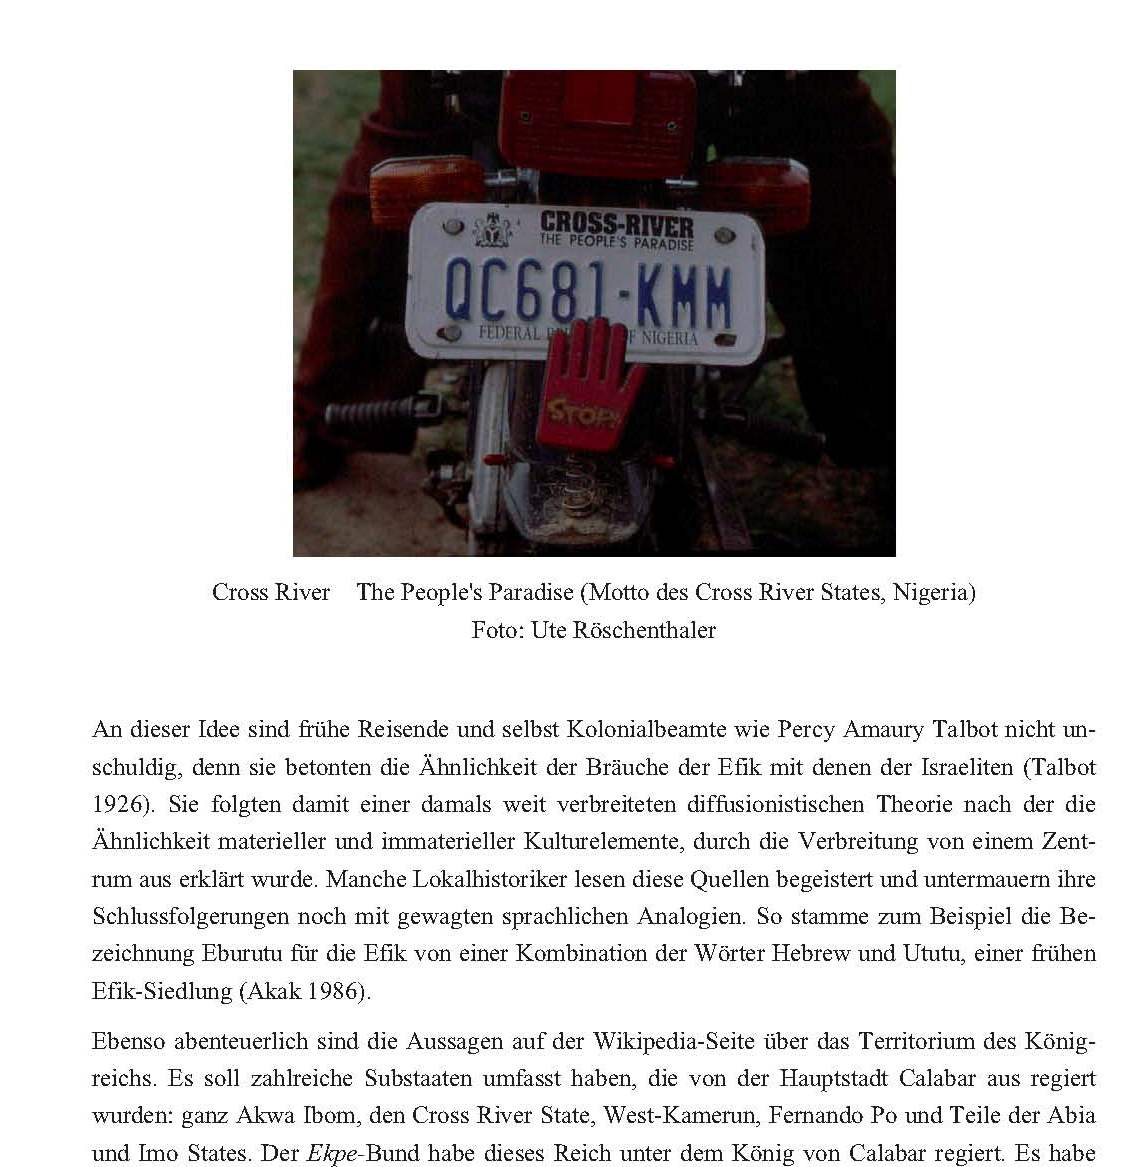
\includegraphics[width=0.5\textwidth]{grafik1.jpg}}
\caption[Beispiel einer Abbildung]{Wie auf der Abbildung von Röschenthaler (2010: 3) zu erkennen ist, wird
die Cross River Region auf den Fahrzeugkennzeichen als \enquote{The People‘s
Paradise} bezeichnet.}
\label{img:grafik1}
\end{figure}

\subsection{Interviews und persönliche Gespräche}

\begin{itemize}
    \item Tonaufnahme
\begin{itemize}
    \item Transkript
\begin{itemize}
        \item teilweise oder vollständig
    \item Archivierung
\end{itemize}
    \item Angabe in Texten als Interviews
\begin{itemize}
    \item Keine Formatvorgabe
\begin{itemize}
    \item Beispiel: (Red Owl 2010: Interview)
\end{itemize}
    \item Detailangaben in Quellenverzeichnis
\begin{itemize}
    \item Beispiel: Red Owl, Richard, 28.7.2010, bei Kyle, SD
\end{itemize}
\end{itemize}
\end{itemize}
    \item Allgemeine Gespräche mit Informanten
\begin{itemize}
    \item im Text mit \enquote{pers. Gespr.} (persönliches Gespräch) statt
    \enquote{Interview} belegt
\end{itemize}
\end{itemize}

\section{Hausarbeit}

\subsection{Der Sinn von Hausarbeiten}

\begin{itemize}
    \item fachspezifische Grundsätze der wissenschaftlichen Kommunikation
    einüben
    \item selbstständig wissenschaftliche Fragestellungen bearbeiten
    \item Argumente logisch und schlüssig darstellen
    \item Methoden oder Theorien des Faches anwenden
    \item Fachliche Konzepte/Begriffe werden korrekt angewendet
    \item Vertrauen in die eigene Kompetenz entwickeln
    \item Anknüpfung an bestehende Forschung
    \item Transparente Darstellung der eigenen Ergebnisse
    \item Schreiben mit klarer Struktur und in verständlichem Schreibstil
    entwickeln
\end{itemize}

\subsection{Formalia}

\begin{itemize}
    \item einheitliche Schriftart
    \item Gut: Times New Roman, Arial, Calibri o.ä.
    \item Schlecht: Bauhaus93, Brush Script, Comic Sans o.ä.
    \item Schriftgrößen: Times 12, Arial 11, Calibri 11
    \item Zeilenabstand: 1,5
    \item Rand links und rechts: 2,5 cm
    \item Blocksatz
    \item Silbentrennung: im Zweifelsfall bei Dozent erfragen
    \item Layout: Einzug bei Absatz, 1,0--1,5 cm
    \item \emph{Alle} Seiten werden gezählt, auch das Deckblatt
    \item Die Nummerierung beginnt erst auf der zweiten Seiten
    \item Angaben zu Seitenumfang (z.B. 10--12 Seiten) beziehen sich in der
    Regel auf den Fließtext
    \item Die Kapitel und Unterkapitel werden nummeriert
\begin{itemize}
    \item[] 1 $\rightarrow$ 1.1, 1.2, 1.3 $\rightarrow$ 1.1.1, 1.1.2, 1.1.3 usw.
    \item[] 2 $\rightarrow$ 2.1, 2.2, 2.3 $\rightarrow$ 2.1.1, 2.1.2, 2.1.3 usw.
\end{itemize}
    \item Regeln des Paraphrasierens, Zitierens und des Belegens von Quellen
    beachten
    \item an den Abgabetermin halten
\end{itemize}

\subsection{Abbildungen}

\begin{itemize}
    \item Abbildungen (Grafiken, Fotos, Karten u.a.) müssen einen inhaltlichen
    Mehrwert bringen
    \item Karten können zur Orientierung wichtig oder gar notwendig sein
    \item Abbildungen müssen durchnummeriert (z.B. Abb. 1, Abb. 2 usw.) werden
    \item Abbildungen müssen eine Bildbeschriftung haben und belegt werden
\end{itemize}

\subsection{Aufbau}

\begin{itemize}
    \item Deckblatt (formale Angaben)
    \item Inhaltsverzeichnis
    \item Einleitung
    \item Hauptteil
    \item Schluss, -folgerung, -bemerkung
    \item Literaturverzeichnis (ggf. Anhänge)
    \item Ehrenwörtliche Erklärung
\end{itemize}

\subsubsection{Deckblatt}

Siehe Abbildung \ref{img:deckblatt} auf Seite \pageref{img:deckblatt}.

\begin{figure}[ht]
\centering
\fbox{
\includegraphics[width=0.95\textwidth,page=1]{Template/example.pdf}}
\caption{Beispiel eines Deckblattes}
\label{img:deckblatt}
\end{figure}

\subsubsection{Inhaltsverzeichnis}

Das Inhaltsverzeichnis soll die Gliederung einer Hausarbeit veranschaulichen,
sowie die ihr zugrunde liegende Argumentation erkenntlich machen. Eine solche
Gliederung besteht immer aus der Einleitung, einem untergliederten Hauptteil,
dem Schluss und einem Literaturverzeichnis (jeweils mit Seitenangaben).Dabei ist
darauf zu achten, dass kein Punkt einer Untergliederung alleine stehen darf
(d.h.: 1.1 nie ohne 1.2).

Siehe Abbildung \ref{img:inhaltsverzeichnis} auf Seite
\pageref{img:inhaltsverzeichnis}.

\begin{figure}[ht]
\centering
\fbox{
\includegraphics[width=0.95\textwidth,page=2]{Template/example.pdf}}
\caption{Beispiel eines Inhaltsverzeichnis}
\label{img:inhaltsverzeichnis}
\end{figure}

\subsubsection{Einleitung}

\begin{itemize}
    \item erläutert den Entstehungskontext der Arbeit
    \item benennt das Thema und kontextualisiert es im wissenschaftlichen
    Diskurs bzw. im Rahmen des Seminarthemas
    \item grenzt das Thema ein
    \item gibt einen Überblick über die Gliederung der Arbeit
    \item gibt Aufschluss über verwendete Literatur oder andere Quellen
\end{itemize}

\subsubsection{Hauptteil}

\begin{itemize}
    \item enthält die Darstellung des Gegenstands der Arbeit
    \item baut das Argument schrittweise und logisch auf
    \item ist untergliedert und mit aussagekräftigen Überschriften versehen
\end{itemize}

\subsubsection{Schluss, -folgerung, -bemerkung}

\begin{itemize}
    \item fasst die Ergebnisse zusammen und zieht einen Schluss aus der
    Darstellung
    \item benennt evtl. die Grenzen der Arbeit
    \item gibt evtl. einen Ausblick auf weiterführende Fragen
\end{itemize}

\subsubsection{Literaturverzeichnis}

\begin{itemize}
    \item Nach den Vorgaben
\begin{itemize}
    \item Alphabetisch
    \item Nicht nach Typen (Internet, Buch, Zeitschrift usw.) sortiert
\end{itemize}
    \item Vollständig
    \item Nur verwendete Literatur
    \item Auch Abbildungsverzeichnis ergänzen
\end{itemize}

\subsubsection{Ehrenwörtliche Erklärung}

\begin{figure}[ht]
\centering
\fbox{
\includegraphics[width=0.95\textwidth,page=19]{Template/example.pdf}}
\caption{Beispiel einer Ehrenwörtlichen Erklärung}
\label{img:ehrenwoertliche_erklaerung}
\end{figure}

Siehe Abbildung \ref{img:ehrenwoertliche_erklaerung} auf Seite
\pageref{img:ehrenwoertliche_erklaerung}.

\subsection{Zitieren und Belegen in Hausarbeiten}

\paragraph{Direkte Zitate:}
Dem Zitat folgt gleich im Fließtext ein Kurzbeleg (Harvard)

\paragraph{Beispiel:}
\begin{quote}
\enquote{Ich bin schon lange der Meinung, daß [sic] Lehre und Studium der
Ethnologie mehr Spaß machen sollten, als es bisher der Fall ist} (Turner 1989:
140).
\end{quote}

komplette bibliographische Angabe erst im Literaturverzeichnis der Hausarbeit:

Literaturverzeichnis:
\begin{quote}
Turner, Victor (1989): \emph{Vom Ritual zum Theater: Der Ernst des menschlichen
Spiels}. Frankfurt: Campus-Verlag.
\end{quote}

\paragraph{Indirekte Zitate:}
siehe direktes Zitat
\paragraph{Beispiel:}

\begin{quote}
Ethnologie sollte im Studium mehr Spaß machen als bisher (Tuner 1989: 140).
\end{quote}

\paragraph{Hinweis:}
Die sogenannte deutsche Zitierweise, der Beleg in einer Fußnote, findet am
Institut für Ethnologie keine Anwendung.

\paragraph{Wie oft belegen?}
Pro Absatz mindestens einmal
\begin{itemize}
\item Wenn mehrere Absätze von derselben Stelle stammen, lohnt es sich
vermutlich inhaltlich sie zusammenzufügen
\item Fragen Sie sich nicht \enquote{Muss ich hier wirklich belegen?}, sondern
\enquote{Muss ich hier wirklich nicht belegen?}
\item Freigestellte Zitate \emph{mit Anführungsstrichen}
\end{itemize}

\newpage
\section{Hilfreiche Literatur}

Antweiler, Christoph (2003): \emph{Ethnologie lesen. Ein Führer durch den Bücher
--Dschungel} (Arbeitsbücher -- Kulturwissenschaft, 1). 3. Aufl. Münster: Lit.

Beer, Bettina und Hans Fischer (2003): \emph{Wissenschaftliche Arbeitstechniken
in der Ethnologie} (Ethnologische Paperbacks). 2. überarb. und erw. Aufl.
Berlin: Reimer.

Beinke, Christiane (2008): \emph{Die Seminararbeit. Schreiben für den Leser.}
Konstanz: UVK--Verl.--Ges.

Eco, Umberto (1993): \emph{Wie man eine wissenschaftliche Abschlussarbeit
schreibt. Doktor-, Diplom und Magisterarbeit in den Geistes- und
Sozialwissenschaften.} 11. Aufl. Heidelberg: C.F.Müller/UTB.

Esselborn--Krumbiegel, Helga (2008): \emph{Von der Idee zum Text. Eine Anleitung
zum wissenschaftlichen Schreiben.} 3. überarb. Aufl. Paderborn: Schoningh
(utb.de--Bachelor--Bibliothek).

Franck, Norbert und Joachim Stary (2009): \emph{Die Technik wissenschaftlichen
Arbeitens. Eine praktische Anleitung.} 15. überarb. Aufl. Paderborn: Schoningh
(UTB).

Frank, Andrea, Haacke, Stefanie und Swantje Lahm (2007):
\emph{Schlüsselkompetenzen. Schreiben in Studium und Beruf.} Stuttgart: Metzler.

Grätz, Frank (2006): \emph{Duden Wie verfasst man wissenschaftliche Arbeiten?
Ein Leitfaden für das Studium und die Promotion.} 3. völlig neu erarb. Aufl.
Mannheim: Bibliographisches Institut.

Krämer, Walter (2009): Wie schreibe ich eine Seminar- oder Examensarbeit?
(campus concret). 3. überarb. Aufl. Frankfurt am Main: Campus.

Kruse, Otto (2007): \emph{Keine Angst vor dem leeren Blatt. Ohne
Schreibblockaden durchs Studium.} 12. völlig neu bearb. Aufl. Frankfurt, New
York: Campus.

Kruse, Otto (2010): \emph{Lesen und Schreiben. Der richtige Umgang mit Texten im
Studium.} Wien: UKV/UTB.

Niederhauser, Jürg (2000): \emph{Duden. Die schriftliche Arbeit. Ein Leitfaden
zum Schreiben von Fach-, Seminarund Abschlussarbeiten in der Schule und beim
Studium; Literatursuche, Materialsammlung und Manuskriptgestaltung mit vielen
Beispielen.} 3. völlig neu erarb. Aufl. Mannheim: Dudenverlag.

Niederhauser, Jürg (2011): \emph{Duden Praxis kompakt - Die schriftliche
Arbeit.} Mannheim: Bibliographisches Institut.

Pospiech, Ulrike (2012): \emph{Duden Ratgeber - Wie schreibt man
wissenschaftliche Arbeiten? Alles Wichtige von der Planung bis zum fertigen
Text.} Mannheim: Bibliographisches Institut.

Sesink, Werner (2003): \emph{Einführung in das wissenschaftliche Arbeiten. Mit
Internet, Textverarbeitung, Präsentation.} 6. völlig überarb. und aktualisierte
Aufl. München: Oldenburg.

Standop, Ewald und Matthias L.G. Meyer (2008): \emph{Die Form der
wissenschaftlichen Arbeit. Grundlagen, Technik und Praxis für Schule, Studium
und Beruf.} 18. bearb. und erw. Aufl. Wiebelsheim: Quelle \& Meyer.

Wolfsberger, Judith (2010): \emph{Frei geschrieben. Mut, Freiheit und Strategie
für wissenschaftliche Abschlussarbeiten.} 3. Aufl. Stuttgart: UTB.

\subsection*{Hilfe}
Allgemeine Schreibberatung: \\Schreibzentrum :
\url{http://www2.uni-frankfurt.de/43403430/Schreibzentrum}

bei mangelnden Deutschkenntnissen:
\begin{itemize}
    \item Hinweis an Dozenten
    \item Schreibberatung des Internationalen Schreibzentrums:
\end{itemize}
\url{http://www.uni-frankfurt.de/international/stk/index.html}

\newpage
\microtypesetup{protrusion=false}
\listoffigures
\newpage
\listoftables
\microtypesetup{protrusion=true}

\newacronym{aao}{a.a.o.}{Am angegebenen Ort}
\newacronym{abb}{Abb.}{Abbildung}
\newacronym{abh}{Abh.}{Abhandlung(en)}
\newacronym{anh}{Anh.}{Anhang}
\newacronym{anm}{Anm.}{Anmerkung}
\newacronym{arch}{Arch.}{Archiv}
\newacronym{aufl}{Aufl.}{Auflage}
\newacronym{ausg}{Ausg.}{Ausgabe}
\newacronym{bd}{Bd. (Bde.)}{Band (Bände)}
\newacronym{beih}{Beih.}{Beiheft}
\newacronym{beitr}{Beitr.}{Beitrag (Beiträge)}
\newacronym{cf}{cf.}{confer = vergleiche}
\newacronym{ders}{Ders.}{derselbe}
\newacronym{dies}{Dies.}{dieselbe}
\newacronym{diss}{Diss.}{Dissertation}
\newacronym{ebd}{ebd., ebda.}{ebenda, an der selben Stelle}
\newacronym{ed}{ed. (Pl. eds.)}{editor(s) = Herausgeber}
\newacronym{einf}{Einf.}{Einführung}
\newacronym{einl}{Einl.}{Einleitung}
\newacronym{ergh}{Erg.H.}{Ergänzungsheft}
\newacronym{ersch}{ersch.}{erschienen}
\newacronym{erw}{erw.}{Erweitert}
\newacronym{etal}{et al.}{et alii = und andere}
\newacronym{f}{f. (Pl.ff.)}{folgende Seite(n)}
\newacronym{fig}{Fig.}{Figur}
\newacronym{fussn}{Fußn.}{Fußnote}
\newacronym{ges}{Ges.}{Gesellschaft}
\newacronym{gesa}{Ges. Ausg.}{Gesamtausgabe}
\newacronym{h}{H.}{Heft}
\newacronym{hgg}{hg.}{herausgegeben}
\newacronym{hg}{Hg., Hrsg.}{Herausgeber}
\newacronym{ibid}{ib., ibid.}{ibidem = ebenda}
\newacronym{ie}{i.e.}{id est = das ist}
\newacronym{j}{J.}{Journal}
\newacronym{jb}{Jb.}{Jahrbuch}
\newacronym{jg}{Jg.}{Jahrgang}
\newacronym{loc}{loc.cit}{loco citato = am angeführten Ort}
\newacronym{ms}{Ms. (Pl.Mss.)}{Manuskript(e)}
\newacronym{nb}{N.B., NB}{Nota bene = beachte}
\newacronym{neudr}{Neudr.}{Neudruck}
\newacronym{nf}{N.F.}{Neue Folge}
\newacronym{ns}{N.S., NS}{New Series = Neue Folge}
\newacronym{oj}{o.J.}{ohne Jahr}
\newacronym{oo}{o.O.}{ohne Ort}
\newacronym{opcit}{op.cit.}{opere citate = im angeführten Werk}
\newacronym{par}{P.}{pars = Teil}
\newacronym{pag}{p. (Pl.pp.)}{pagina = Seite(n)}
\newacronym{pa}{p.a.}{pro anno = jährlich}
\newacronym{reg}{Reg.}{Register}
\newacronym{repr}{Repr.}{Reproduktion, Neudruck}
\newacronym{s}{S.}{Seite}
\newacronym{ser}{Ser.}{Serie}
\newacronym{slg}{Slg.}{Sammlung}
\newacronym{suppl}{Suppl., suppl.}{Supplement = Ergänzung(-sband), Nachtrag}
\newacronym{ua}{u.a.}{und andere}
\newacronym{vgl}{vgl.}{vergleiche}
\newacronym{vs}{vs.}{versus = gegen, gegenüber}
\newacronym{wb}{Wb.}{Wörterbuch}
\newacronym{z}{Z., Zs., Zeitschr.}{Zeitschrift}
\newacronym{ziff}{Ziff.}{Ziffer}

\glsaddall

\newpage
\begin{multicols}{2}
    \printacronyms[title={Abkürzungsverzeichnis}]
\end{multicols}

\end{document}
